\documentclass[12pt]{article}

\usepackage{sbc-template}
\usepackage{ragged2e}
\usepackage{graphicx,url}
\usepackage{tikz}
%\usepackage[brazil]{babel}   
\usepackage[utf8]{inputenc}
\usepackage{xcolor,listings}
\usepackage{hyperref}

\hypersetup{
	colorlinks=true,
    linkcolor=,
    filecolor=purple,
    urlcolor=blue,
    citecolor=pink,
}




% Default fixed font does not support bold face
\DeclareFixedFont{\ttb}{T1}{txtt}{bx}{n}{12} % for bold
\DeclareFixedFont{\ttm}{T1}{txtt}{m}{n}{12}  % for normal

% Custom colors
\usepackage{color}
\definecolor{deepblue}{rgb}{0,0,0.5}
\definecolor{deepred}{rgb}{0.6,0,0}
\definecolor{deepgreen}{rgb}{0,0.5,0}


% Python style for highlighting
\newcommand\pythonstyle{\lstset{
language=Python,
basicstyle=\small,
otherkeywords={self},             % Add keywords here
keywordstyle=\ttb\color{deepblue},
emph={MyClass,__init__},          % Custom highlighting
emphstyle=\ttb\color{deepred},    % Custom highlighting style
stringstyle=\color{deepgreen},
frame=tb,                         % Any extra options here
showstringspaces=false            % 
}}


% Python environment
\lstnewenvironment{python}[1][]
{
\pythonstyle
\lstset{#1}
}
{}

% Python for external files
\newcommand\pythonexternal[2][]{{
\pythonstyle
\lstinputlisting[#1]{#2}}}

% Python for inline
\newcommand\pythoninline[1]{{\pythonstyle\lstinline!#1!}}
\pagenumbering{alph}
\def\checkmark{\tikz\fill[scale=0.4](0,.35) -- (.25,0) -- (1,.7) -- (.25,.15) -- cycle;}
\sloppy

% Tallys: Acho que o nome do padrão poderia ser Exception Handling Pattern
\title{Clear Exception Message Pattern}

\author{Eduardo Delgado Coloma Bier\inst{1}, Fernanda de Camargo Magano\inst{1}, \\ Fernando Freire Scattone\inst{1},
  Florence Alyssa Sakuma Shibata\inst{1}, Tallys Gustavo Martins\inst{1} }

\address{Instituto de Matemática de Estatística -- Universidade de São Paulo
  (USP)
  \email{\{eduardo.bier,fernanda.magano,fernando.scattone,florence.shibata\}@usp.br}
  \email{tallys@ime.usp.br}
}

\pagenumbering{roman}

\begin{document} 

\maketitle

\begin{abstract}

 
 Dealing with exceptions is an important part of many applications, they can happen anywhere at anytime during the code execution --- from assigning a variable to opening a network connection. From a software developer's point of view, handling this the right way might not be so trivial, because aspects like code quality, cohesion and modularity should be taken into account when writing exceptions, specially in big projects. Therefore, using a pattern for the exception messages forces the developer to think about the exceptions they may encounter and write them down in a modular way, so that newcomers to the project can easily identify their errors. This paper shows the ``Clear Exception Message Pattern'' developed by the authors, exposing the strengths and weaknesses, as well as known usages and the pattern format.
 
%Dealing with exceptions is an important part of many applications, they can happen anywhere at anytime during the code execution, from assigning a variable to opening a network connection. From the sight of a software developer, handling this exceptions in the correct way might not be so trivial, because there are some aspects like code quality, cohesion and modularity that should be taken into account, especially in big projects. Therefore, using a pattern for the exception messages brings consistency to the code and allows reuse inside of the same application or among different ones. The current paper shows the ``Clear Exception Message Pattern'' developed by the authors, exposing the strengths and weaknesses, as well as known usages and the pattern format \cite{smith:99}, \cite{bernardo2008importancia}.

%Writing clear exception messages is useful for solving problems in the code faster, because the source of the issues are stated in a clear manner. Therefore, using a pattern for the exception messages brings consistency to the code and allows reuse inside of the same application or among different ones, since dealing with exceptions is an important part of every application. 
  
\end{abstract}


\section{Introduction}

When developing a system, quality code is desirable to solve the proposed problems and meet the requirements. However, as the system becomes more complex, it is harder to isolate and fix bugs and errors. The ability to detect, diagnose and handle these issues is essential to the maintenance and support of the final product. By using mechanisms such as logging and writing clear and meaningful exceptions, developers can detect errors as soon as they occur and obtain sufficient information about them to quickly fix problems in the code.

If errors are handled incorrectly, they can reduce the usability of the system. For example, users might think an application is unreliable if exceptions are not handled properly, specially if they are not worded in a very clear way. These messages are also very important for programmers, because if an exception isn't clear, they will need more time to find and fix bugs, leading to extra costs for the company they work for or even to users. \\

\begin{python}[caption="Generic error given by the language",captionpos=b,label="generic_error"] 
class Calculator:
	def __init__(self, value):
		self.value = value
	def getCalculator():
		return None
	def sum(self, a, b):
		self.value = a + b
		return self.value

b = Calculator.getCalculator()
b.sum(2, 3)
\end{python}

In the example above, the program would throw the following error: 
\begin{verbatim}
AttributeError: 'NoneType' object has no attribute 'sum'
\end{verbatim} \hfill \newline
As one can see, that message is not that helpful, unless the programmer knows Python really well and has a clear idea of where the problem might be in the code. By writing richer exception messages, however, developers can get much better information. The following example shows a better way to handle this exception, using the Clear Exception Message Pattern. \\

\begin{python}[breaklines=true,caption="Treatment of exception",captionpos=b] 
class NoneCalculatorException(Exception):
	def __init__(self, message):
		self.message = "This calculator doesn't exist. " + message
		super().__init__(self.message)

c = Calculator.getCalculator()
if c == None:
	raise NoneCalculatorException("The sum cannot occur because the variable is None.")
else:
	c.sum(2, 3)
\end{python}

In this case, the thrown exception would be: 

\begin{verbatim}
NoneCalculatorException: This calculator doesn't exist. 
The sum cannot occur because the variable is None.
\end{verbatim}
This is a much more detailed exception message, that will probably help the developer find and fix the problem quickly.

Even though there is a large variety of languages for developing applications, there is no standard documentation for handling exceptions or errors. Each developer is responsible for generating some sort of mechanism for capturing and handling these cases. Aiming to simplify and fix bugs more easily we proposed the Clear Exception Message Pattern that seeks a standard way to write messages in exceptions that are not too long but, at the same time, are sufficiently expressive to easily understand what the problem is and where it occurred.

This pattern can be used in projects of different domains, since catching exceptions is fundamental in every application developed in real world scenarios. It brings consistency and consequently allows the reuse of code.\cite{1687854} was used as a main source of information, alongside \cite{smith:99} and \cite{bernardo2008importancia}.

\section{Pattern}

\begin{flushleft}
\textbf{Name:} Clear Exception Message Pattern \\
\end{flushleft}

\begin{flushleft}
\textbf{Type:} Structural \\
\end{flushleft}

\begin{flushleft}
\textbf{Intent:} Write exception messages that are specific to the domain of the application and easier to understand.\\
\end{flushleft}

\begin{flushleft}
\textbf{Motivation:}
When writing applications it is necessary to catch and treat exceptions that may arise. But developers might not have all the technical expertise to understand all the exceptions from the programming language, so it is convenient to deal with exceptions that can better indicate where the error occurred to reduce the time wasted in debugging activities.\\
\end{flushleft}

\begin{flushleft}
\textbf{Also Known As:} Error Message Pattern, Formatted Message Pattern\\
\end{flushleft}

\begin{flushleft}
\textbf{Pattern format description:}
\end{flushleft}

\begin{figure}[!htb]
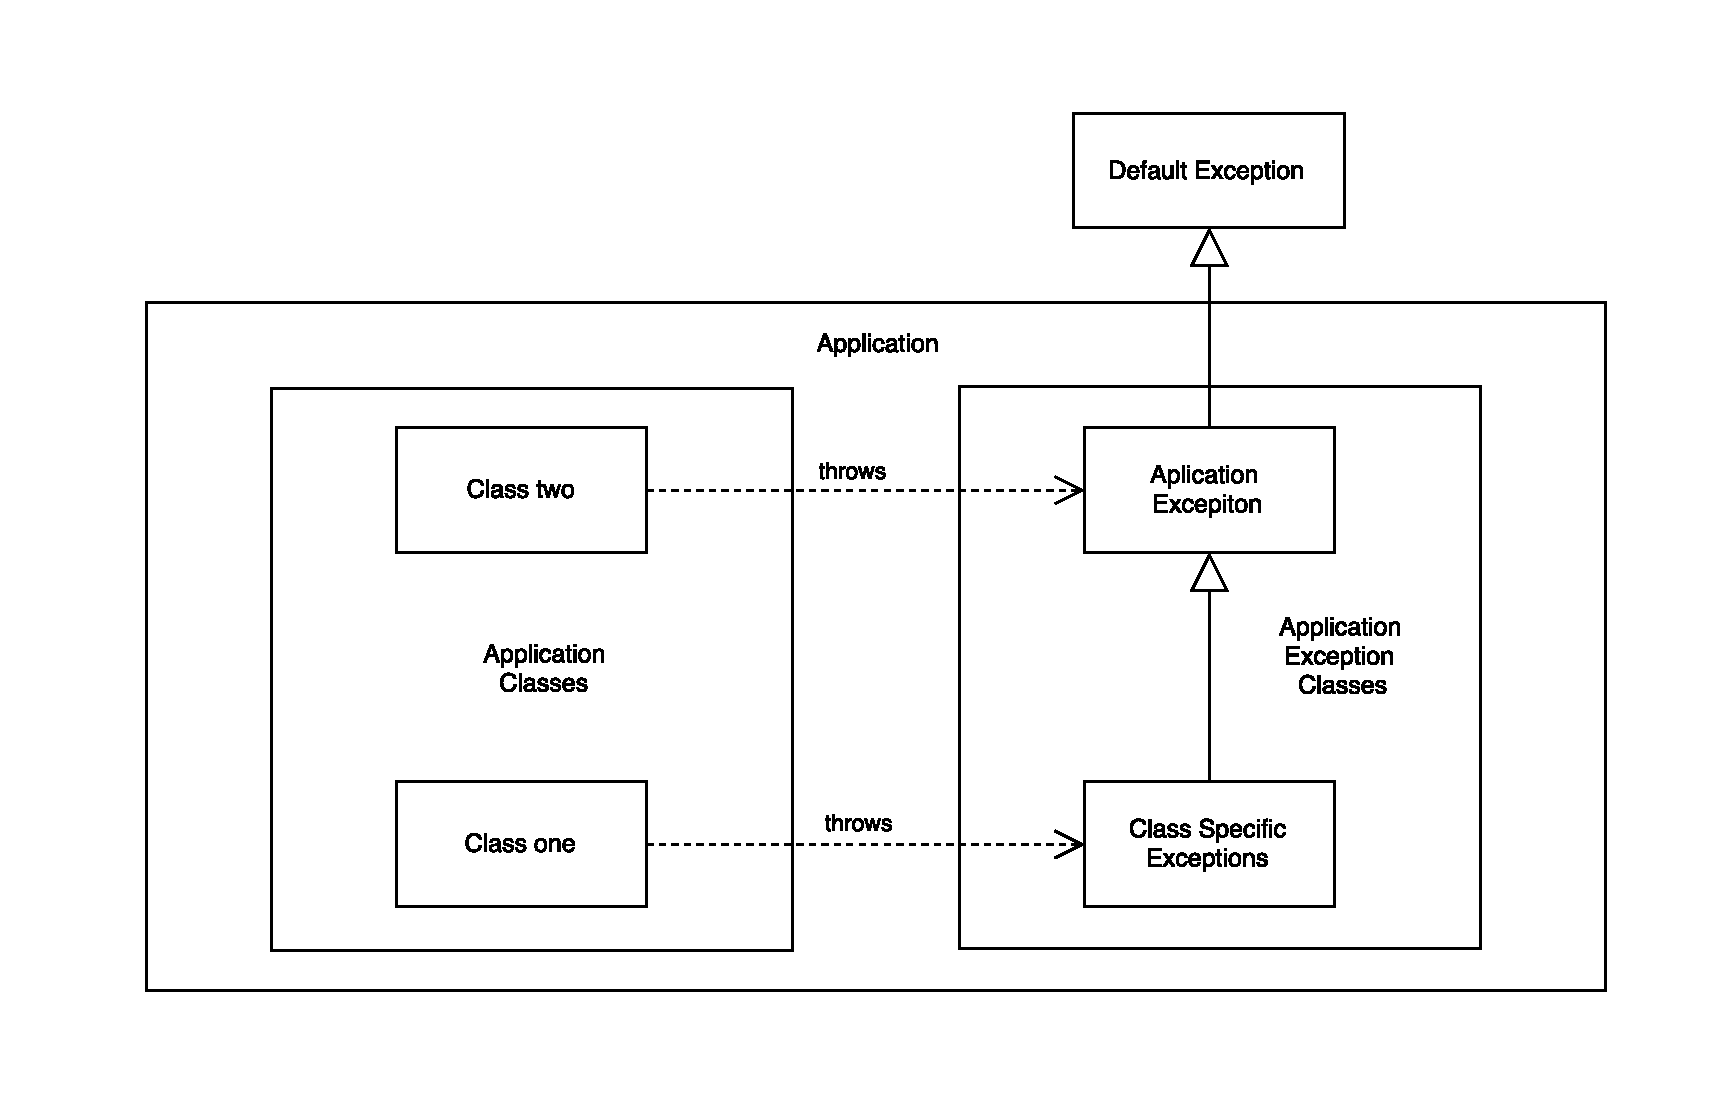
\includegraphics[width=\textwidth]{diagrama.pdf}
\caption{UML diagram of Clear Exception Message Pattern}
\label{UML-diagram}
\end{figure}

Figure \ref{UML-diagram} shows two application classes. In order to implement the Clear Exception Message Pattern it's necessary to create, at least, an Application Exception Class, which will treat exceptions that may appear on most classes of the application. If needed, specific classes of the application may have their own class-specific exception class, that will inherit all common exception treatments from the Application Exception Class. 

\newpage
The Clear Exception Message Pattern deals with specific kinds of exception handling messages such as:
 \begin{enumerate}
 \item Exception with files
 \item Exception with connection status
 \item Incompatible variable types 
  \end{enumerate} 
 
The first one treats common problems with files, like: not found, wrong permissions -- try to write in a file opened for reading. The second deals with connection issues. The pattern gives the example of failure to open TCP connection, but other possible issues are timeout, connection forbidden, among others. The last item refers to problems with conversion of types -- if the program sums numbers but among the variables are strings, for example.

The more generic an exception is, the harder it is to find errors in the code, so it's very important that caught exceptions are as specific as possible. Therefore, one of the goals of this pattern is writing exceptions that cover very specific situations.
 
One exception has some information associated with it. Among them are the error type, the cause, the trace and they help to understand the exception itself. As a result, the pattern messages will contain information about the type of the exception, a brief description and, where appropriate, some information about the trace like the line number where the exception occurred.
\newline

\begin{flushleft}
\textbf{Antagonic Forces:} 
\end{flushleft} 
When running an application, developers might encounter exceptions that might be hard to interpret or might not pinpoint the culprit of the problem. This usually happens because programming languages only have exceptions for very generic cases that encompass various specific cases, which make it harder for developers to find issues in their code. This is aggravated in large projects, where this may happen often and bugs are even harder to find due to the project's size.  \newline


\begin{flushleft}
\textbf{Strengths:} 
\end{flushleft}

\begin{enumerate}
\item Messages will follow a pattern and will be similar to each other, making them consistent throughout the code.

\item It provides succinct information of the error increasing the quality and readability of the code.

\item It is easier for other programmers that didn’t program the application to understand how the codes works.

\item It helps the maintenance of the application and it's lifecycle management.

\item Informing specific error message allows robust framework implementation and program flow monitoring.

%\textbf{[CASO NOSSO CÓDIGO TENHA TEMPLATE (algum lugar que centralize o tratamento de erros) - CASO NÃO TENHA, RETIRAR ESTE ITEM!]}
\item The improvement of exception handling later in the development process can be done easily in a single spot. \\ \\ \newline

\end{enumerate}

\begin{flushleft}
\textbf{Weaknesses:}
\end{flushleft}

\begin{enumerate}
\item The amount of work dedicated to finding possible exceptions that may occur might be too much to handle, depending on the team working the code, time constraints, and scale of the project.

\item There is a possibility of re-throwing exceptions (chaining exceptions) causing loss of efficiency.
\end{enumerate}%\textbf{Fernando}\newline 

\begin{flushleft}
\textbf{Consequences:}
\end{flushleft}

\begin{enumerate}
%
\item Time and energy in finding errors will be reduced
\item Whenever the context is similar, it is possible to reuse the set of written exception messages in the same application or even in different projects, thus reducing effort.
\item By implementing specific exceptions for all cases the modularization of the software is improved, since each module will have a clear and separated function.
\item The pattern forces the developer to think about the exceptions for each class, which may help them better understand the project and see if the requirements are being delivered.
\end{enumerate}

\begin{flushleft}
\textbf{Known usages:}
\end{flushleft}

Some prestigious languages such as Ruby and Python, already come with very detailed exception by default.\newline


\begin{flushleft}
\textbf{Recommended usage:}
\end{flushleft}

\begin{enumerate}
\item Large projects where new people are joining and the production environment could be made a little bit friendlier by helping new programmers find their errors.
\item Medium projects where the team is always changing and new members are not very familiar with the language they are using.
\end{enumerate} 
%\textbf{Tallys}



\begin{flushleft}
\textbf{Discouraged usage:}
\end{flushleft}

\begin{enumerate}
\item The project is too small - The time and energy required to implement the pattern may not be worth it.
%\item The people who developed the software from the start are the same ones as in production. In this case, they are very familiar with the code and maybe they don't need this pattern in order to know where the exception appear.
\end{enumerate}

\begin{flushleft}
\textbf{Code examples:}
\end{flushleft}
We decided to write code examples in Java and Ruby to illustrate that the Clear Exception Message Pattern can be used in both compiled and dynamic languages. The complete code is in the appendix.

\begin{flushleft}
\textbf{Related Patterns:}
\end{flushleft}

The Clear Exception Message is an exception pattern and it is possible to find other similar patterns in the \href{http://wiki.c2.com/?ExceptionPatterns}{wiki}~\footnote{http://wiki.c2.com/?ExceptionPatterns}. 
Among the patterns presented in this page, we can cite one of them that is related to ours, the ``Refine Exceptions''. It is about getting information of particular categories of exceptions and throw the most specific ones, which is a key part of our pattern, since exception messages should be as clear as possible.
The ``Clear Exception Message'' is also related with GoF Template Method, but the difference between them is that our pattern doesn't necessarily have a fixed structure, i.e. the message is flexible and can be changed according to the context of the application.

\section{Conclusion}

The developed pattern treats specific exception handling messages, like file not found, connection issues, since the more specific the caught exception is, the clearer is the source of the problem. The readability of the messages, the possibility of code reuse and the ease of maintaining the system are the main goals of this pattern.


\bibliographystyle{sbc}
\bibliography{sbc-template}
\newpage

\appendix
\section{Appendix}
\lstinputlisting[language=Ruby, caption=clear\_exceptions.rb]{codd.rb}
\lstinputlisting[language=Java, caption=Exceptions.java, basicstyle=\small, breaklines=true]{Exceptions.java}
\end{document}
